\section{Results}
\subsection{Simulation: GridWorld}

Gridworld is a commonly used environment in the study of reinforcement learning \cite{RL}. Our version of GridWorld is set up as a simple maze, where the agent needs to find the quickest route to the exit.
It is typically represented as a two-dimensional matrix, where each cell in the grid corresponds to a different state that an agent could be in. We used GirdWorld as a toy environment to learn an optimal policy via Q-learning.

Our agent begins at the most top left corner cell, and learns moving from one cell to another, in order to reach the final cell at the bottom right corner. The agent can choose from 4 actions: up, down, left, or right.

States or cells in the grid  have different properties. All cells excepts the final cell at the bottom right corner give the agent a reward of -1, the final cell (end state) give the agent a reward of +1. This reward structure forces  the agent  to find the quickest route to the exit.

Our implementation of GirdWorld takes in 5 user-defined hyper parameters, can be easily modified at the begin of the program. Different hyperparameters in the Q-learning algorithm can impact the agent's learning performance and overall behavior. Here's an overview of the hyperparameters and how they can influence the agent based on our experiments and literature:
\begin{enumerate}[(i)]
    \item \textbf{Learning rate} $\alpha$: This parameter determines how much the agent updates its Q-values based on new information. A high learning rate means the agent gives more importance to recent experiences, while a low learning rate indicated it relies more on its accumulated knowledge. We found if the learning rate was set too high, the agent sometimes failed to converge or learned a suboptimal policy. If it's set too low, the ``learning process"  was slow or the agent may get stuck in a local optimum .

    \item \textbf{Discount factor} $\gamma$: As discussed earlier, this parameter determines how much the agent values future rewards compared to immediate rewards. High discount factor means the agent puts more emphasis on long-term rewards, while a low discount factor makes the agent more focused on short-term rewards. If the discount factor is too high, the agent may take longer to learn an optimal policy, as it needs to explore more steps into the future. If it's too low, the agent may learn a suboptimal policy that only focuses on short-term gains.
    
    \item \textbf{Initial Exploration rate} $\epsilon$: This parameter determines the initial probability that the agent chooses a random action instead of the action with the highest Q-value \cite{RL}. A high exploration rate means the agent explores the environment more, while a low exploration rate means the agent focuses more on exploiting its current knowledge. If the exploration rate is too high, the agent took longer to learn an optimal policy, as it spends more time exploring. If it is set too low, the agent may not explore enough to find the best actions and learn a suboptimal policy.

    \item \textbf{Exploration Decay rate}: This parameter determines how fast the exploration rate decreases over time. A high decay rate means the agent reduces its exploration rate quickly, while a low decay rate means the agent maintains a higher exploration rate for longer. We found if the decay rate is too high, the agent may not explore enough to learn an optimal policy. If it was set too low, the agent took longer to converge, as it continued to explore even when it has already learned a good policy.

    \item \textbf{Number of raining episodes} $n$ : This parameter sets the total number of episodes the agent goes through. We found if we set the number of episodes too low, the agent may not have enough time to learn an optimal policy. And if we set it too high, the agent wasted computational resources without significant improvements in performance.

\end{enumerate} 
Tuning these hyperparameters essentially comes down to finding a balance between exploration and exploitation, learning speed and stability, and short-term and long-term rewards. We can use techniques like grid search, random search, or Bayesian optimization to find the optimal combination of hyperparameters for this specific problem, however, exploration of this will be outside the scope of this paper.

\begin{figure}\label{result}
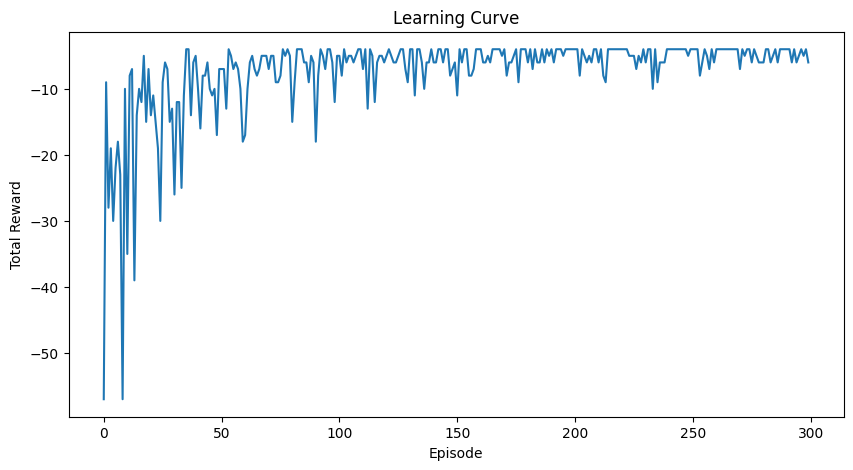
\includegraphics[width=12cm]{lectures/diagrams/result.png}
\centering
\caption{Result from simulation of GridWorld}
\end{figure}
\subsection{Conclusion}
We conclude our discussion with a Figure (2) that provides concrete evidence that our agent is indeed capable of learning a policy that exhibits improvement over successive episodes. As can be clearly observed in the graph, there is a notable increase in the total reward, on average, as the number of episodes escalates. This trend of increasing total reward signifies the agent's progressive learning and adaptation.

The occasional downward spikes in the graph represent instances where the agent chooses to take ``exploratory" actions as opposed to the optimal or ``greedy" action. This is a crucial part of the learning process, allowing the agent to explore a broader range of possible actions and outcomes, thus avoiding the potential pitfall of premature convergence on a suboptimal policy.

Over time, it is observable that the probability of these ``exploratory" actions diminishes, which is indicative of the agent settling into an optimal policy. As a consequence, the total return exhibits greater stability, with fluctuations becoming increasingly infrequent and minor. This illustrates the agent's successful adaptation and the maturing of its learned policy, reinforcing the validity of our approach.


 
